\documentclass{article}
\usepackage{graphicx}
\title{Project Report}
\author{TEAM MARAUDERS\\
		Shaan Vaidya 150050004\\
		Abhishek Kumar 150050020\\
		Vishwajeet Singh Bagdawat 150050046\\
		}
\date{\today}
\begin{document}

	\maketitle

\newpage

\section{Django backend}
	The backend for the API is built using Django framework. The backend basically provides features of Instructors to effectively manage the courses and take feedbacks from students. The django server is managed completely by an administrator who has rights to add students and courses to the web API. The instructor registers into the app either normally through the interface of the app or through facebook login.
\newline
\newline
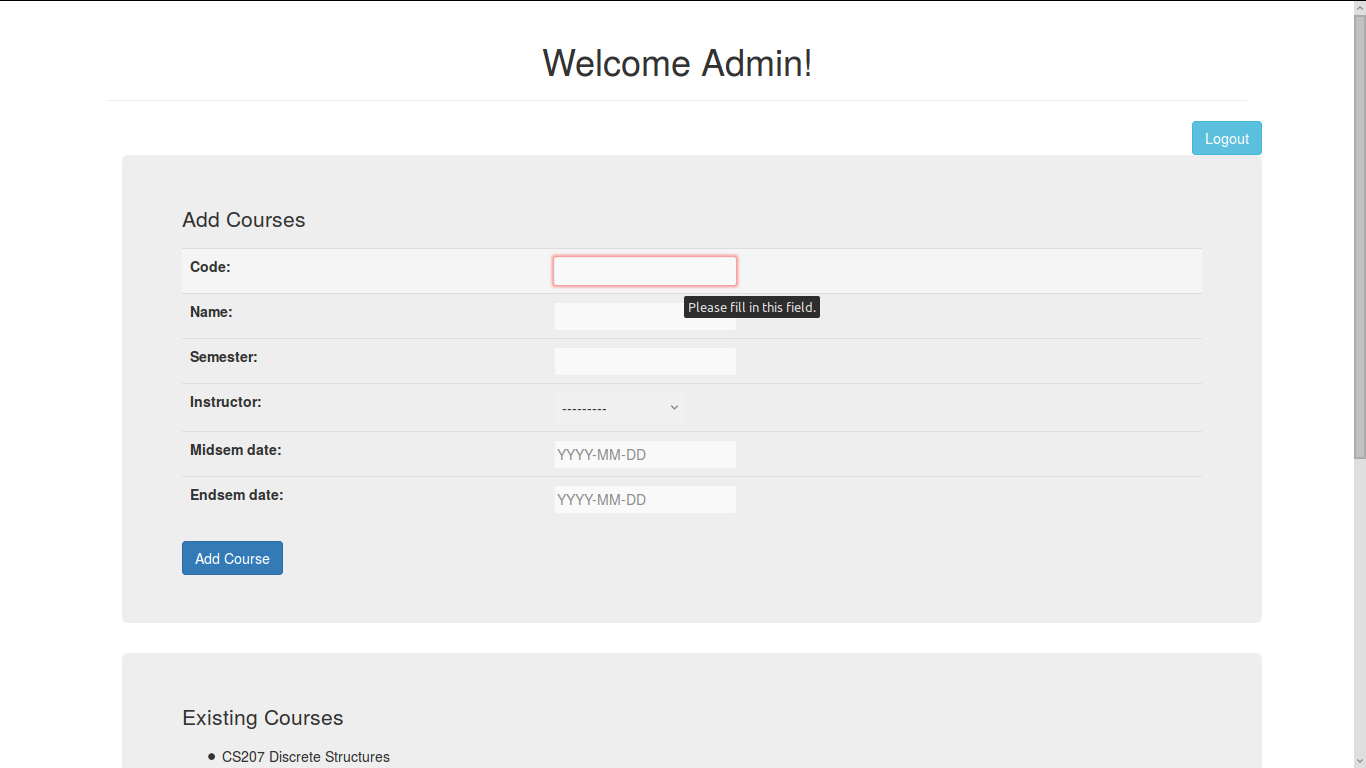
\includegraphics[width=15cm, height=10cm]{photos/addcourse.png}

	The instructors can then add deadlines and feedback forms.
	We assume that all instructors are honest and trustworthy and can see each other's deadlines, forms and feedbacks
\newpage
\section{Features:}
\begin{itemize}
\item Addition of courses and students by the admin
\item Login and register options for instructors including sign up through facebook
\item Creating feedback forms by the instructors having dynamic number of rows
\item Adding deadlines for assignments and exams
\end{itemize}
\hfill \break
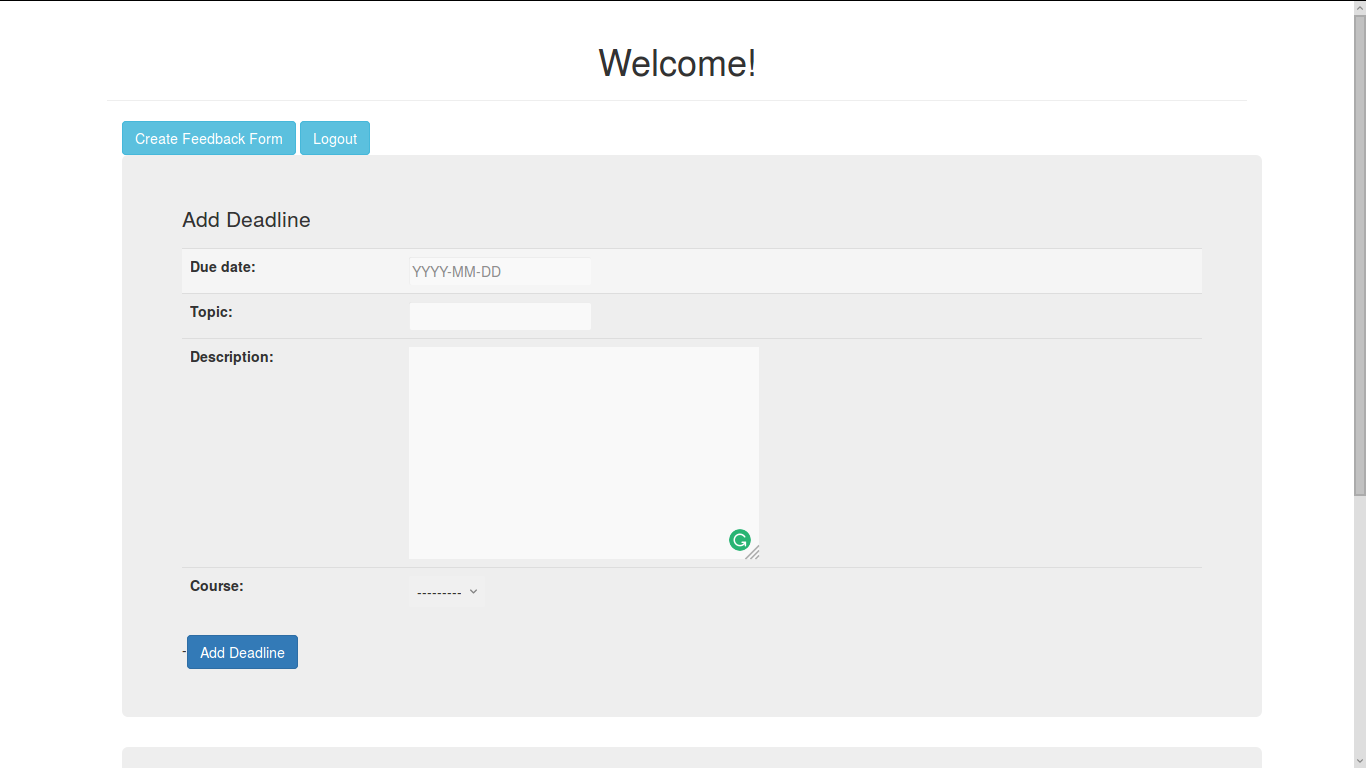
\includegraphics[width=15cm, height=10cm]{photos/deadline.png}
\newpage
\section{Android Frontend}
	The Android App is built using Android Studio. The Feeder App provides the students a easy way to manage their deadlines provided by the instructors. The App provides a login page and logout button. Even if the app is closed after logging in and then reopened the user remains logged in.
\\
\hfill \break
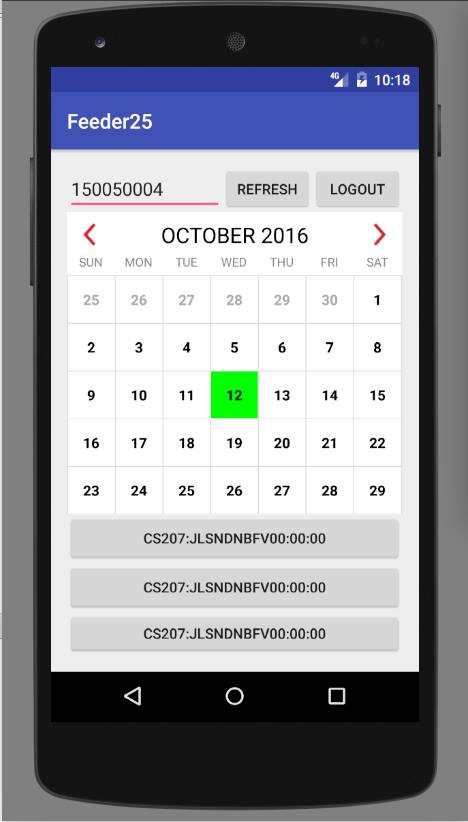
\includegraphics[width=8cm, height=14cm]{photos/android.png}
\newpage
\section{Features:}
\begin{itemize}
\item Logging into app by authenticating from the backend 
\item Getting information about the courses of a student, deadlines and feedback
\item Viewing the deadlines in the calender
\end{itemize}
\hfill \break
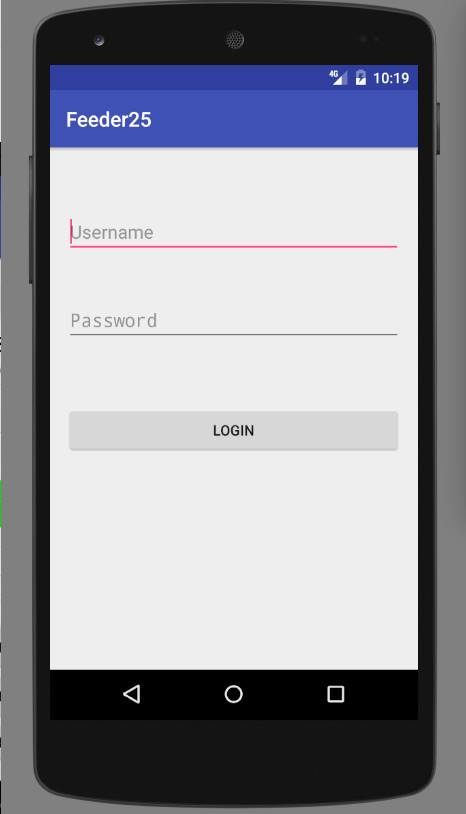
\includegraphics[width=8cm, height=14cm]{photos/android2.png}
\newpage
\section{Important notes for running the app:}
\begin{itemize}
\item While registering through facebook the user would be kept logged in until he logs out of the original facebook account from the browser
\item While adding questions in adding feedback forms you can add both rating type questions as well as subjective type questions 
\item The deadlines are separately displayed into two types- The ones which are upcoming and the ones which are over
\end{itemize}
\hfill \break	
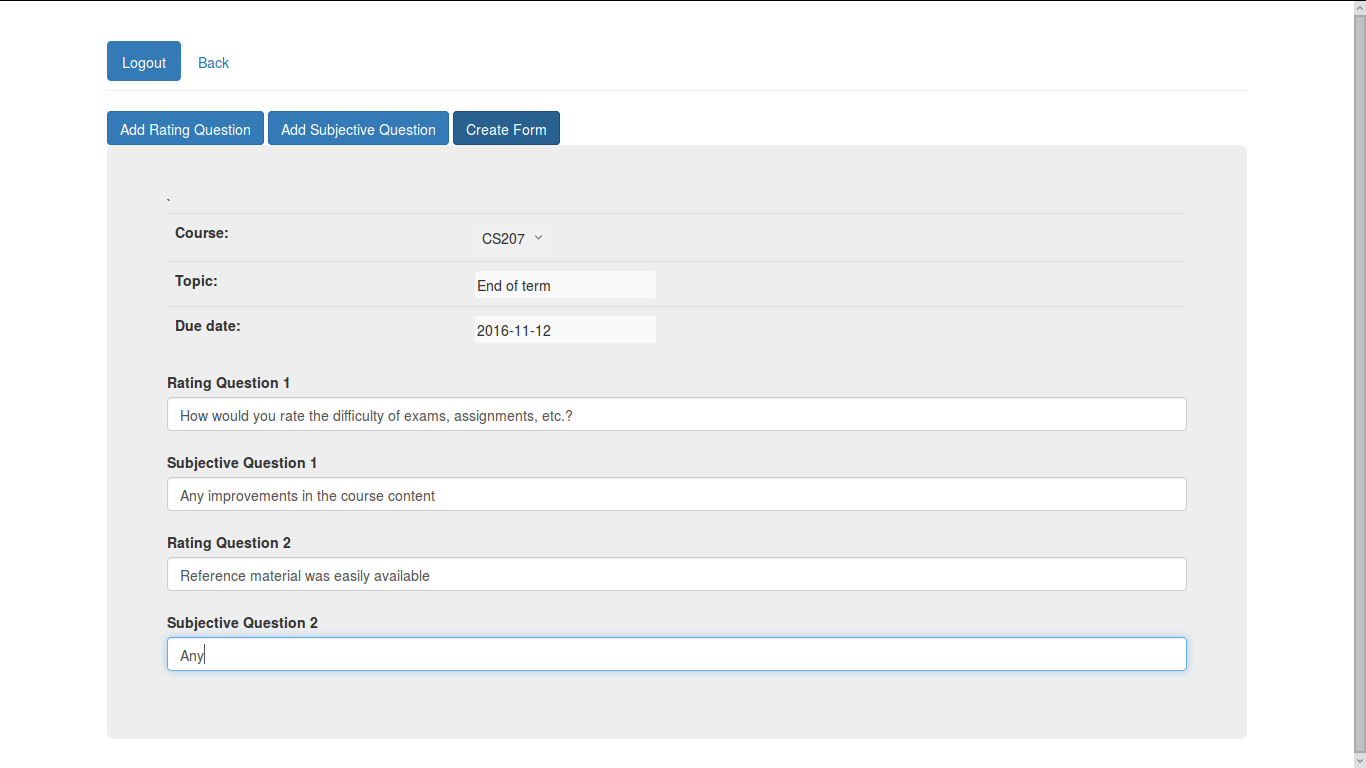
\includegraphics[width=15cm, height=10cm]{photos/feedback.png}
\newpage
\section{Reflections}
The project was the one thing we worked the most on in this course. At face value, learning a plethora of new things would seem quite daunting and so it did. But once the structure of how things worked became clearer, it was just a matter of finding the correct ways to do things.\\
\hfill \break	
Django was perhaps the easier of the two, at least for us. Android Studio did keep giving random pains, but once we figured out what the errors were, they didn't feel so random, in fact, such pedanticism about things is the reason that working apps are so stable because otherwise there is an infinite number of things that could go wrong and one would never know about it. Django was fun! Creating models, relating them, passing data between views, etc.\\ 
\hfill \break	
We do regret that we weren't able to accomplish all of the features and we apologise for it. It was sheer incompetence on our part that led to our not being able to complete the whole thing in the stipulated time. We learnt a lot (first thing being, BEGIN EARLY!) in the course of the project.\\
\hfill \break	
All in all, the whole course has been a enriching journey. When we look back, we find that we are much more confident in walking into untested waters now than we were before. Bring it on!\\
\hfill \break	
We also thank the whole teaching team for the course, for making it so much fun!\\
\hfill \break	
It all ends here, one would say, but I would argue that this is in fact a new beginning!
\end{document}